\documentclass[12pt]{a&t}
\pdfminorversion=4

%\usepackage[utf8]{inputenc}
%\usepackage[T2A]{fontenc}
\usepackage{graphics,graphicx}
\usepackage[normalem]{ulem}
%\usepackage{slashbox}
\usepackage[usenames]{color}
%\usepackage{colortbl}
%\usepackage[noend]{algorithmic}
%\usepackage{a4wide}
%\usepackage{amsthm}
%\usepackage[english,russian]{babel}
%\usepackage[all]{xy}
\usepackage{subfig}
%\usepackage{subfigure}
\usepackage{cmap}
%\usepackage{caption}																							
%\usepackage{subcaption}
%\usepackage{caption}
%\usepackage{subcaption}
%\newtheorem*{theorem*}{Theorem}
%\usepackage{ntheorem}
%\newtheorem*{theorem_empty}{\hspace{\parindent}\sl{Т\,е\,о\,р\,е\,м\,а\,}}

%\renewcommand\theassump{A\arabic{assump}}
\DeclareMathOperator*{\argmax}{arg\,max}
\DeclareMathOperator*{\argmin}{arg\,min}
\begin{document}
\year{2018}
\title{ВЫБОР МОДЕЛЕЙ ГЛУБОКОГО ОБУЧЕНИЯ СУБОПТИМАЛЬНОЙ СЛОЖНОСТИ}
\thanks{Работа выполнена при поддержке Российского фонда фундаментальных исследований (проект 16-37-00488) и РФ (соглашение № 05.Y09.21.0018).}
\authors{О.Ю.~БАХТЕЕВ (bakhteev@phystech.edu)\\ 
(Московский физико-технический институт),\\
В.В. СТРИЖОВ, д-р физ.-мат. наук (strijov@phystech.edu)\\
(Вычислительный центр им. А.А. Дородницына ФИЦ ИУ РАН)}

\maketitle




\begin{abstract}Рассматривается задача выбора моделей глубокого обучения субоптимальной сложности. Под сложностью модели понимается минимальная длина описания совокупности выборки и модели классификации или регрессии. Под субоптимальной сложностью понимается приближенная оценка минимальной длины описания, полученная с использованием байесовского вывода и вариационных методов. Вводятся вероятностные предположения о распределении параметров. На основе байесовского вывода предлагается функция правдоподобия модели. Для получения оценки правдоподобия применяются вариационные методы с использованием градиентных алгоритмов оптимизации. Проводится вычислительный эксперимент на нескольких выборках.
\end{abstract}

\textit{Ключевые слова:} классификация, регрессия, глубокое обучение, выбор модели, байесовский вывод, вариационный вывод, сложность.
\section{Введение}

Проблема выбора модели является одной из ключевых задач машинного обучения. Под моделью понимается суперпозиция функций, решающая задачу классификации или регрессии.
В данной работе в качестве критерия выбора модели предлагается субоптимальная сложность модели. Под сложностью модели понимается \emph{минимальная длина описания}~\cite{mdl}, т.е. минимальное количество информации, которое требуется передать о модели и о выборке. Вычисление минимальной длины описания модели является вычислительно сложной процедурой. В работе предлагается получение ее приближенной оценки, основанной на связи минимальной длины описания и \emph{правдоподобия модели}~\cite{mdl}. {В общем случае данная величина является трудновычислимой.} Для получения оценки правдоподобия используются вариационные методы получения оценки правдоподобия~\cite{Bishop}, основанные на аппроксимации неизвестного другим заданным распределением. Под субоптимальной сложностью понимается вариационная оценка правдоподобия модели.


%В работе~\cite{perekrestenko} рассматривается ряд критериев сложности моделей глубокого обучения и их взаимосвязь. В работе~\cite{vladis} в качестве критерия сложности модели выступает показатель нелинейности, характеризуемый степенью полинома Чебышева, аппроксимирующего функцию. В работе~\cite{need_prune} анализируется показатель избыточности параметров сети. Утверждается, что по небольшому набору параметров в глубокой сети с большим количеством избыточных параметров возможно спрогнозировать значения остальных. В работе~\cite{rob} рассматривается показатель робастности моделей, а также его взаимосвязь с топологией выборки и классами функций, в частности рассматривается влияние функции ошибки и ее липшицевой константы на робастность моделей. Схожие идеи были рассмотрены в работе~\cite{intrig}, в которой исследуется устойчивость классификации модели под действием шума. 
%В ряде работ~\cite{MacKay,Bishop,tokmakova,zaitsev,strijov_webber, strijov_dsc} в качестве критерия выбора модели  выступает правдоподобие модели. В работах~\cite{tokmakova,zaitsev,strijov_webber, strijov_dsc} рассматривается проблема выбора модели и оценки гиперапараметров в задачах регрессии. Альтернативным критерием выбора модели является минимальная длина описания~\cite{mdl}, являющаяся показателем статистической сложности модели и заданной выборки. В работе~\cite{grun} рассматриваются различные модификации и интерпретации минимальной длины описания, в том числе связь с правдоподобием модели.

Одним из методов получения приближенного значения правдоподобия модели является вариационный метод получения нижней оценки правдоподобия~\cite{Bishop}. % В работе~\cite{hoffman} рассматривается стохастическая версия вариационного метода.
В~\cite{nips} рассматривается алгоритм получения вариационной нижней оценки правдоподобия  для оптимизации гиперпараметров моделей глубокого обучения. 
%В работе~\cite{varmc} рассматривается взаимосвязь градиентных методов получения вариационной нижней оценки интеграла с методом Монте-Карло.
В~\cite{early} рассматривается стохастический градиентный спуск в качестве оператора, порождающего распределение, аппроксимирующее апостериорное распределение параметров модели. В работе отмечается, что стохастический градиентный спуск не оптимизирует вариационную оценку правдоподобия, а приближает ее только до некоторого числа итераций оптимизации. 
%Схожий подход рассматривается в работе~\cite{sgd_cont}, где также рассматривается стохастический градиентный спуск в качестве оператора, порождающего апостериорное распределение параметров. В работе~\cite{langevin} предлагается модификация стохастического градиентного спуска, аппроксимирующая апостериорное распределение. 


%Альтернативным методом выбора модели является выбор модели на основе скользящего контроля~\cite{cv_ms, tokmakova}. Проблемой такого подхода является возможная высокая вычислительная сложность~\cite{expensive, expensive2}. В работах~\cite{bias,bias2} рассматривается проблема смещения оценок качества модели и гиперпараметров, получаемых при использовании $k$-fold метода скользящего контроля, при котором выборка делится на $k$-частей с обучением на $k-1$ части и валидацией результата на оставшейся части выборки. 


%Задачей, связанной с проблемой выбора модели, является задача оптимизации гиперпараметров~\cite{MacKay,Bishop}. В работе~\cite{hyperopt} рассматривается оптимизация гиперпараметров с использованием метода скользящего контроля и методов оптимизации интеграла правдоподобия моделей, отмечается низкая скорость сходимости гиперпараметров при использовании метода скользящего контроля. В работах~\cite{hyper, hyper2} рассматриваются градиентные методы оптимизации гиперпараметров, позволяющие оптимизировать большое количество гиперпараметров одновременно. В работе~\cite{hyper} предлагается метод оптимизации гиперпараметров с использованием градиентного спуска с моментом. В качестве оптимизируемого функционала рассматривается ошибка на валидационной части выборки.  В работе~\cite{early} отмечается возможность использовать градиентный метод для оптимизации гиперпараметров с использованием вариационной нижней оценки интеграла правдоподобия в качестве оптимизируемого функционала.

Одна из проблем построения моделей глубокого обучения --- большое число параметров модели~\cite{hinton_rbm}, которое достигает нескольких миллионов, а оптимизация модели достигает десятков дней~\cite{suts}. Задача выбора модели глубокого обучения включает в себя выбор стратегии построения модели, эффективной по вычислительным ресурсам. 
%В работе~\cite{sgd_cont} рассматривается задача оптимизации параметров градиентного спуска с использованием нижней вариационной оценки интеграла правдоподобия.


%В работе~\cite{greed} приводятся теоретические оценки построения нейросетей с использованием жадных стратегий,  при которых построение модели производится итеративно последовательным увеличением числа нейронов в сети. В работе~\cite{greed_mlp} предлагается жадная стратегия выбора модели нейросети с использованием релевантных априорных распределений, т.е. параметрических распределений, оптимизация параметров которых позволяет удалить часть параметров из модели. Данный метод был к задаче построения модели метода релевантных векторов~\cite{rvm}. Альтернативой данным алгоритмам построения моделей являются методы, основанные на прореживании сетей глубокого обучения~\cite{obd, popova}, т.е. последовательного удаления параметров, не дающих существенного прироста качества модели. 
%В работах\cite{Bengio, hd} рассматривается послойное построение модели с отдельным критерием оптимизации для каждого слоя. В работах~\cite{Kingma, gendis_pictures, gendis_phd} предлагается декомпозиция модели на порождающую и разделяющую, оптимизируемых последовательно. 

%В качестве порождающих моделей в сетях глубокого обучения выступают ограниченные машины Больцмана~\cite{hinton_rbm} и автокодировщики~\cite{founds}. В работе~\cite{contractive} рассматриваются алгоритмы регуляризации автокодировщиков, позволяющих формально рассматривать данные модели как порождающие модели с использованием байесового вывода. В работе~\cite{score} рассматриваются регуляризованные автокодировщики и свойства оценок их правдоподобия. В работе~\cite{vae} предлагается обобщение автокодировщика с использованием вариационного байесовского вывода~\cite{Bishop}. В работе~\cite{train_generative} рассматриваются модификации вариационного автокодировщика и ступенчатых сетей~\cite{ladder} для случая построения многослойных порождающих моделей. 


В данной работе предлагается метод получения вариационной нижней оценки  правдоподобия модели с использованием модифицированного алгоритма стохастического градиентного спуска. {Модификация заключается в добавлении шумовой компоненты. Эта компонента позволяет получить более точные оценки правдоподобия модели для сравнения моделей и выбора наиболее адекватной из них. } Рассматривается ряд модификаций базового алгоритма. {В качестве базового алгоритма выступает алгоритм оптимизации параметров модели с использованием стохастического градиентного спуска без контроля переобучения. Он заключается в итеративном вычислении градиента по параметрам от функции правдоподобия обучающей выборки и изменении значений параметров с его учетом.} Приводится сравнение с алгоритмом получения вариационной нижней оценки, представленном в~\cite{nips}. {Рассматриваются следующие модификации базового алгоритма:
%\begin{enumerate}
%\item 
оптимизация с кросс-валидацией с использованием и без использования регуляризации модели,
алгоритм получения вариационной оценки правдоподобия модели с применением нормального распределения,
алгоритм получения вариационной оценки правдоподобия с использованием стохастического градиентного спуска,
алгоритм получения вариационной оценки правдоподобия с использованием стохастической динамики Ланжевена.}
 { Данные алгоритмы решают следующие проблемы оптимизации моделей  градиентным спуском: оптимизация модели с меньшими затратами вычислительных ресурсов, быстрая сходимость оптимизации, контроль переобучения и выбор наиболее адекватной модели.
Под переобучением понимается потеря обобщающей способности модели с увеличением правдоподобия обучающей выборки~\cite{MacKay}. Переобучение характерно для моделей с большим количеством параметров, сопоставимым с мощностью обучающей выборки, что встречается в случае выбора моделей глубокого обучения~\cite{hinton_rbm, suts}.
}
Также алгоритмы имеют дальнейшую возможность применения к градиентным алгоритмам оптимизации гиперпараметров, описанным в~\cite{hyper}.

Свойства представленных в данной работе  алгоритмов исследуется на выборках, на которых проверялась работа алгоритма вероятностного обратного распространения ошибок~\cite{pbp}, где авторы акцентируются на оптимизации параметров модели. 


\section{Постановка задачи оптимизации правдоподобия модели}
Задана выборка  \begin{equation}\label{eq:dataset}\mathfrak{D} = \{(\mathbf{x}_i,y_i)\}, i = 1,\dots,m,\end{equation} состоящая из множества пар <<объект-метка>> $$\mathbf{x}_i \in \mathbf{X} \subset \mathbb{R}^n, \quad {y}_i \in \mathbf{y} \subset \mathbb{Y}.$$ Метка ${y}$  объекта $\mathbf{x}$ принадлежит либо множеству: ${y} \in \mathbb{Y} = \{1, \dots, Z\}$ в случае задачи классификации, где $Z$ --- число классов, либо некоторому подмножеству вещественных чисел ${y} \in \mathbb{Y}  \subseteq \mathbb{R}$ в случае задачи регрессии.

Моделью глубокого обучения $\mathbf{f}$ назовем суперпозицию функций
\begin{equation}
\label{eq:main}
 \mathbf{f}(\mathbf{w}, \mathbf{X}) = \mathbf{f}_1(\mathbf{f}_2(\dots \mathbf{f}_K(\mathbf{w}, \mathbf{X}))): \mathbb{R}^{m \times n} \to \mathbb{Y}^m,
\end{equation}
где $\mathbf{f}_k$ --- подмодели, параметрическое семейство дважды дифференцируемых по параметрам вектор-функций, $k \in \{1,\dots,K\}$; $\mathbf{w} \in \mathbb{R}^u$~---~вектор параметров моделей.\\
Для каждой модели определена функция правдоподобия  $p(\mathbf{y}|\mathbf{X}, \mathbf{w}, \mathbf{f})$, где $\mathbf{x}$ --- строка матрицы $\mathbf{X}$, $\mathbf{y}$ --- вектор меток зависимой переменной $y$.
Множество всех рассматриваемых моделей обозначим $\mathfrak{F}$. Для каждой модели $\mathbf{f}$ из конечного множества моделей $\mathfrak{F}$ задано априорное распределение параметров $p(\mathbf{w}|\mathbf{f})$.

%http://arxiv.org/pdf/math/0406221v1.pdf
\begin{definition} Сложностью модели $\mathbf{f}$ назовем правдоподобие модели: %стохастическую сложность ее описания~\cite{mdl, grun2}:
%\[
%	\textnormal{C}(\mathbf{y},\mathbf{f}) = \textnormal{Len}(\mathbf{y}|\hat{\mathbf{w}}, \mathbf{f}) + \textnormal{COMP}(\mathbf{f}),
%\]
%где  $\textnormal{Len}(\mathbf{y}|\hat{\mathbf{w}}, \mathbf{f})$ --- \emph{длина описания} матрицы $\mathbf{y}$ с использованием модели $\mathbf{f}$ и оценки вектора %параметров $\hat{\mathbf{w}}$, полученных методом наибольшего правдоподобия, а $\textnormal{COMP}(\mathbf{f})$ --- величина, характеризующая \emph{параметрическую сложность} модели, т.е. способность модели описать произвольную выборки из $\mathbb{R}^n$~\cite{grun}.

%Байесовой интерпретацией сложности $\textnormal{C}$ является правдоподобие модели~\cite{MacKay}:
\begin{equation}
\label{eq:evidence}
	p(\mathbf{y}|\mathbf{X},\mathbf{f}) = \int_{\mathbf{w} \in \mathbb{R}^u} p(\mathbf{y}|\mathbf{X},\mathbf{w}, \mathbf{f})p(\mathbf{w}|\mathbf{f})d\mathbf{w}.
\end{equation}
\end{definition}
Модели $\mathbf{f} \in \mathfrak{F}$ имеют различные размерности $u$ соответствующих векторов параметров. Также заданы различные априорные распределения их параметров $p(\mathbf{w}|\mathbf{f})$.
%Заметим, что в общем случае оценки правдоподобия модели и сложности модели могут различаться~\cite{grun}.


\begin{definition}Модель классификации $\mathbf{f}$ назовем оптимальной среди моделей $\mathfrak{F}$, если достигается максимум интеграла~\eqref{eq:evidence}.
\end{definition}


Требуется найти оптимальную модель $\mathbf{f}$ среди заданного множества моделей $\mathfrak{F}$, а также значения ее параметров $\mathbf{w}$, доставляющие максимум апостериорной вероятности
\begin{equation}
\label{eq:posterior}
	p(\mathbf{w}|\mathbf{y},\mathbf{X},\mathbf{f}) = \frac{p(\mathbf{y}|\mathbf{X}, \mathbf{w}, \mathbf{f})p(\mathbf{w}|\mathbf{f})}{p(\mathbf{y}|\mathbf{X}, \mathbf{f})}.
\end{equation}


%\begin{example_empty}
\textsl{П\,р\,и\,м\,е\,р~\,1.} Рассмотрим задачу линейной регрессии:
\[
	\mathbf{y} =\mathbf{X} \mathbf{w} + \boldsymbol{\varepsilon},\quad \boldsymbol{\varepsilon}  \sim \mathcal{N}(\mathbf{0},\mathbf{1}),\quad \mathbf{w} \sim  \mathcal{N}(\mathbf{0},\mathbf{A}^{-1}),
\]
где $\mathbf{A}$ --- диагональная матрица. 
Правдоподобие зависимой переменной имеет вид
\begin{equation}
\label{eq:example1}
	p(\mathbf{y}|  \mathbf{X}, \mathbf{w}, \mathbf{f}) = (2\pi) ^{-\frac{m}{2}} \textnormal{exp} \bigl(-\frac{1}{2}(\mathbf{y} -\mathbf{X} \mathbf{w})^\mathsf{T}(\mathbf{y} - \mathbf{X}\mathbf{w})\bigr),
\end{equation}
априорное распределение параметров модели имеет вид
\begin{equation}
\label{eq:prior}	
p(\mathbf{w}|\mathbf{f}) =  (2\pi) ^{-\frac{n}{2}} |\mathbf{A}|^{\frac{1}{2}} \textnormal{exp} (-\frac{1}{2}\mathbf{w}^\mathsf{T}\mathbf{A}\mathbf{w}).
\end{equation}

Правдоподобие модели~\eqref{eq:evidence} в этом примере вычисляется аналитически~\cite{hyperopt}:
\begin{equation}
\label{eq:ground}
	p(\mathbf{y}|\mathbf{X},\mathbf{f})  =  (2\pi) ^{-\frac{m}{2}} |\mathbf{A}|^{\frac{1}{2}} |\mathbf{H}|^{-\frac{1}{2}}  \textnormal{exp}\bigl(-\frac{1}{2}(\mathbf{y} -\mathbf{X} \hat{\mathbf{w}})^\mathsf{T}(\mathbf{y} - \mathbf{X}\hat{\mathbf{w}})\bigr)\textnormal{exp} \bigl(-\frac{1}{2}\hat{\mathbf{w}}^\mathsf{T}\mathbf{A}\hat{\mathbf{w}}\bigr),
\end{equation}
где $\hat{\mathbf{w}}$ --- значение наиболее вероятных~\eqref{eq:posterior} параметров модели:
\[
	\hat{\mathbf{w}} = \argmax p(\mathbf{w}|\mathbf{y}, \mathbf{X}, \mathbf{f}) = (\mathbf{A} + \mathbf{X}^\mathsf{T}\mathbf{X})^{-1}\mathbf{X}^\mathsf{T}\mathbf{y},
\]
$\mathbf{H}$ --- гессиан функции потерь $L$ модели:
\[
	\mathbf{H}	= \nabla \nabla_\mathbf{w} \left(\frac{1}{2} (\mathbf{y} -\mathbf{X} {\mathbf{w}})^\mathsf{T}(\mathbf{y} - \mathbf{X}{\mathbf{w}}) + \frac{1}{2}\mathbf{w}^\mathsf{T}\mathbf{A}\mathbf{w} \right) = \mathbf{A} + \mathbf{X}^\mathsf{T}\mathbf{X},
\]

\[ 
	L = - \textnormal{log} p(\mathbf{y}|  \mathbf{X}, \mathbf{w}, \mathbf{f}). 
\]
%\end{example_empty}

%\paragraph{Пример 2.} Рассмотрим задачу классификации, в которой модель --- нейросеть с softmax-слоем на выходе:
%\[
%\mathbf{f} = \mathbf{f}_\textnormal{SM}(\mathbf{f}_2(\dots \mathbf{f}_K(\mathbf{x}))),
%\]
%$\mathbf{f}_2, \dots, \mathbf{f}_K$ --- дифференцируемые функции, $\mathbf{f}_\textnormal{SM}$ --- многомерная логистическая функция:
%\[
%	\mathbf{f}_\textnormal{SM} = \frac{\mathbf{f}_2(\dots \mathbf{f}_K(\mathbf{x}))}{\sum_{r=1}^Z \textnormal{exp}\bigl( {f}_{r,2}(\dots \mathbf{f}_K(\mathbf{x})) \bigr)},
%\]
%где ${f}_{r,2}$ --- $r$-я компонента функции $\mathbf{f}_2$. Компонента $r$ вектора $\mathbf{f}_\textnormal{SM}$ определяет вероятность принадлежности объекта $\mathbf{x}$ к классу $r$. Логарифм правдоподобия зависимой переменной аналогично~\eqref{eq:example1} имеет вид
%\[
%	\textnormal{log} p({y}|\mathbf{x}, \mathbf{w}, \mathbf{f}) =  \textnormal{log}~\hat{f}_{\hat{r},\textnormal{SM}} (\mathbf{f}_2(\dots \mathbf{f}_K(\mathbf{x}))),
%\]
%где $\hat{f}_{\hat{r},\textnormal{SM}}$ соответствует ненулевой компоненте вектора ${y}$:
%$$\hat{r} \in \{1,\dots,Z\}: y_{r} >0,$$
%$y_{r}$ --- компонента вектора ${y}$. 

%-Интеграл правдоподобия~\eqref{eq:evidence} модели является трудновычислимым для данного семейства моделей. Одним из методов вычисления приближенного значения правдоподобия является получение вариационной оценки правдоподобия.  


{В качестве функции, приближающей логарифм интеграла~\eqref{eq:evidence}, будем рассматривать его нижнюю оценку, полученную при помощи неравенства Йенсена~\cite{Bishop}. Получим нижнюю оценку логарифма правдоподобия модели, используя неравенство}
\begin{equation} 
\label{eq:elbo}
\textnormal{log}~p(\mathbf{y}|\mathbf{X},\mathbf{f})  = \int_{\mathbf{w}} q(\mathbf{w})\textnormal{log}~\frac{p(\mathbf{y},\mathbf{w}|\mathbf{X},\mathbf{f})}{q(\mathbf{w})}d\mathbf{w} + \textnormal{D}_\textnormal{KL}  \bigl(q(\mathbf{w})||p(\mathbf{w}|\mathbf{y}, \mathbf{X}, \mathbf{f})\bigr) \geq	
\end{equation} 
$$
\geq \int_{\mathbf{w}} q(\mathbf{w})\textnormal{log}~\frac{p(\mathbf{y},\mathbf{w}|\mathbf{X},\mathbf{f})}{q(\mathbf{w})}d\mathbf{w} =
$$

$$
= -\textnormal{D}_\textnormal{KL} \bigl(q(\mathbf{w})||p(\mathbf{w}|\mathbf{f})\bigr) + \int_{\mathbf{w}} q(\mathbf{w})\textnormal{log}~{p(\mathbf{y}|\mathbf{X},\mathbf{w},\mathbf{f})} d \mathbf{w},
$$
где $\textnormal{D}_\textnormal{KL}\bigl(q(\mathbf{w})||p(\mathbf{w} |\mathbf{f})\bigr)$ --- расстояние Кульбака--Лейблера между двумя распределениями: $$\textnormal{D}_\textnormal{KL}\bigl(q(\mathbf{w})||p(\mathbf{w} |\mathbf{f})\bigr) = -\int_{\mathbf{w}} q(\mathbf{w})\textnormal{log}~\frac{p(\mathbf{w} | \mathbf{f})}{q(\mathbf{w})}d\mathbf{w},$$
$$
p(\mathbf{y},\mathbf{w}|\mathbf{X},\mathbf{f}) = p(\mathbf{y}|\mathbf{X},\mathbf{f})p(\mathbf{w}|\mathbf{f}).
$$

{
\begin{definition} Вариационной оценкой логарифма правдоподобия модели~\eqref{eq:evidence} $\textnormal{log}~p(\mathbf{y}|\mathbf{X},\mathbf{f})$ называется оценка $\textnormal{log}~\hat{p}(\mathbf{y}|\mathbf{X},\mathbf{f})$, полученная аппроксимацией неизвестного апостериорного распределения $p(\mathbf{w}| \mathbf{y}, \mathbf{X}, \mathbf{f})$ заданным распределением $q(\mathbf{w})$.
\end{definition}
}


Будем рассматривать задачу нахождения вариационной оценки как задачу оптимизации. Пусть задано множество распределений $Q =\{q(\mathbf{w})\}$. Сведем задачу нахождения наиболее близкой вариационной нижней оценки интеграла~\eqref{eq:evidence} к оптимизации вида
\[
     \hat{q}(\mathbf{w}) = \argmax_{q \in Q}  \int_{\mathbf{w}} q(\mathbf{w})\textnormal{log}~\frac{p(\mathbf{y},\mathbf{w}|\mathbf{X},\mathbf{f})}{q(\mathbf{w})}d\mathbf{w}.
\]  
В данной работе в качестве множества $Q$ рассматривается нормальное распределение и распределение параметров, неявно получаемое оптимизацией градиентными методами. 

Оценка~\eqref{eq:elbo} является нижней, поэтому может давать некорректные оценки для правдоподобия~\eqref{eq:evidence}. Для того, чтобы оценить величину этой ошибки, докажем следующее утверждение.

\begin{statement}\label{st:st1} Пусть задано множество $Q = \{q(\mathbf{w})\}$ непрерывных распределений. Максимизация вариационной нижней оценки $$\int_{\mathbf{w}} q(\mathbf{w})\textnormal{log}~\frac{p(\mathbf{y},\mathbf{w}|\mathbf{X},\mathbf{f})}{q(\mathbf{w})}d\mathbf{w}$$  логарифма интеграла~\eqref{eq:evidence}  эквивалентна минимизации расстояния Кульбака--Лейблера между распределением $q(\mathbf{w}) \in Q$ и апостериорным распределением параметров $p(\mathbf{w}|\mathbf{y}, \mathbf{X}, \mathbf{f})$:
\begin{equation}
\label{eq:optim}
    \hat{q} = \argmax_{q \in Q} \int_{\mathbf{w}} q(\mathbf{w})\textnormal{log}~\frac{p(\mathbf{y},\mathbf{w}|\mathbf{X},\mathbf{f})}{q(\mathbf{w})}d\mathbf{w} \Leftrightarrow 	
    \hat{q} = \argmin_{q \in Q} \textnormal{D}_\textnormal{KL}  \bigl(q(\mathbf{w})||p(\mathbf{w}|\mathbf{y}, \mathbf{X}, \mathbf{f})\bigr),
\end{equation}

\[
	\textnormal{D}_\textnormal{KL}  \bigl(q(\mathbf{w})||p(\mathbf{w}|\mathbf{y}, \mathbf{X}, \mathbf{f})\bigr) =  \int_\mathbf{w} q(\mathbf{w}) \frac{q(\mathbf{w})}{p(\mathbf{w}|\mathbf{y}, \mathbf{X}, \mathbf{f})} d\mathbf{w}.
\]

\end{statement}


Таким образом, задача нахождения вариационной оценки, близкой к значению интеграла~\eqref{eq:evidence} сводится к поиску распределения $\hat{q}$, аппроксимирующего распределение $p(\mathbf{w}|\mathbf{y}, \mathbf{X}, \mathbf{f})$ наилучшим образом. Доказательство утверждения~1 см. в Приложении.

\begin{definition} Модель $\mathbf{f}$ назовем субоптимальной на множестве моделей $\mathfrak{F}$  по множеству распределений ${Q}$, если модель доставляет максимум нижней вариационной оценке интеграла~\eqref{eq:optim}
\begin{equation}
\label{eq:elbo2}
	\max_{q \in {Q}}\int_{\mathbf{w}} q(\mathbf{w})\textnormal{log}~\frac{p(\mathbf{y},\mathbf{w}|\mathbf{X},\mathbf{f})}{q(\mathbf{w})}d\mathbf{w}.
\end{equation}
\end{definition}

{
Субоптимальность модели может быть также названа вариационной оптимальностью модели или LB-оптимальностью (\textit{Lower Bound --- нижняя граница}) модели.}

Вариационная оценка~\eqref{eq:elbo} интерпретируется как оценка сложности модели по принципу минимальной длины описания~\cite{mdl}, где первое слагаемое определяет количество информации для описания выборки, а второе слагаемое --- длину описания самой модели~\cite{nips}.
%\[
%	\textnormal{MDL}(\mathbf{y},\mathbf{f}) = \textnormal{Len}(\mathbf{y}|\hat{\mathbf{w}}, \mathbf{f}) + \textnormal{COMP}(\mathbf{f}),
%\]
%где  $\textnormal{Len}(\mathbf{y}|\hat{\mathbf{w}}, \mathbf{f})$ --- \emph{длина описания} матрицы $\mathbf{y}$ с использованием модели $\mathbf{f}$ и оценки вектора %параметров $\hat{\mathbf{w}}$, полученных методом наибольшего правдоподобия, а $\textnormal{COMP}(\mathbf{f})$ --- величина, характеризующая \emph{параметрическую сложность} модели, т.е. способность модели описать произвольную выборки из $\mathbb{R}^n$~\cite{grun}.


В данной работе решается задача выбора субоптимальной модели при различных заданных множествах $Q$.

\section{Методы получения вариационной оценки правдоподобия}
Ниже представлены методы получения вариационных нижних оценок~\eqref{eq:elbo2} правдоподобия~\eqref{eq:evidence}. В первом подразделе рассматривается метод, основанный на аппроксимации апостериорного распределения $p( \mathbf{w}|\mathbf{y}, \mathbf{X}, \mathbf{f})$~\eqref{eq:posterior} многомерным гауссовым распределением с диагональной матрицей ковариаций. В последующих разделах рассматриваются методы, основанные на различных модификациях стохастического градиентного спуска. 

\subsection{Аппроксимация нормальным распределением}
В качестве множества $Q = \{q(\mathbf{w})\}$ задано параметрическое семейство нормальных распределений с диагональными матрицами ковариаций:
\begin{equation}
\label{eq:diag}
	q \sim \mathcal{N}(\boldsymbol{\mu}_q, \mathbf{A}^{-1}_q),
\end{equation}
где $\mathbf{A}_q$ --- диагональная матрица ковариаций, $\boldsymbol{\mu}_q$ --- вектор средних компонент.

Пусть априорное распределение $p(\mathbf{w}|\mathbf{f})$~\eqref{eq:prior} параметров модели задано как нормальное:
\[
	p(\mathbf{w}|\mathbf{f}) \sim \mathcal{N}(\boldsymbol{\mu}, \mathbf{A}^{-1}).
\] 
Тогда оптимизация~\eqref{eq:optim} имеет вид
\begin{equation}
\label{eq:norm_max}
 \int_{\mathbf{w}} q(\mathbf{w})\textnormal{log}~{p(\mathbf{y}|\mathbf{X},\mathbf{w},\mathbf{f})} d \mathbf{w} - D_\textnormal{KL}\bigl(q (\mathbf{w} )|| p (\mathbf{w}|\mathbf{f})\bigr) \to \max_{\mathbf{A}_q, \boldsymbol{\mu}_q},
\end{equation}
где расстояние $D_\textnormal{KL}$ между двумя гауссовыми величинами рассчитывается как 
\[
	D_\textnormal{KL}\bigl(q (\mathbf{w}) || p (\mathbf{w}|\mathbf{f})\bigr) = \frac{1}{2} \bigl( \textnormal{Tr} [\mathbf{A}\mathbf{A}^{-1}_q] + (\boldsymbol{\mu} - \boldsymbol{\mu}_q)^\mathsf{T}\mathbf{A}(\boldsymbol{\mu} - \boldsymbol{\mu}_q) - u +\textnormal{ln}~|\mathbf{A}^{-1}| - \textnormal{ln}~|\mathbf{A}_q^{-1}| \bigr).
\]
В качестве приближенного значения интеграла $$\int_{\mathbf{w}} q(\mathbf{w})\textnormal{log}~{p(\mathbf{y}|\mathbf{X},\mathbf{w},\mathbf{f})} d \mathbf{w}$$ предлагается использовать формулу
\[
\int_{\mathbf{w}} q(\mathbf{w})\textnormal{log}~{p(\mathbf{y}|\mathbf{X},\mathbf{w},\mathbf{f})} d \mathbf{w} \approx \sum_{i=1}^m \textnormal{log}~p({y}_i|\mathbf{x}_i, \mathbf{w}_i),
\]
где $\mathbf{w}_i$  --- реализация случайной величины из распределения $q(\mathbf{w})$.

Итоговая функция оптимизации~\eqref{eq:norm_max} имеет вид
\begin{equation}
\label{eq:gaus}
	\mathbf{f} = \argmax_{\mathbf{A}_q, \boldsymbol{\mu}_q} \sum_{i=1}^m \textnormal{log}~p({y}_i|\mathbf{x}_i, \mathbf{w}_i) - D_\textnormal{KL}\bigl(q (\mathbf{w} )|| p (\mathbf{w}|\mathbf{f})\bigr).
\end{equation}

%\begin{example_empty} 
%\hspace{\parindent}
\textsl{П\,р\,и\,м\,е\,р~\,2.}
Пусть  задана выборка $\mathfrak{D}$, в которой переменная ${y}$ не зависит от $\mathbf{x}$:
\begin{equation}
\label{eq:example_post}
	{y} \sim \mathcal{N}(\mathbf{w}, \mathbf{B}^{-1}),
\end{equation}

\[
	\mathbf{B}^{-1} = \left( \begin{array}{cc}
	2 & 1,8 \\
	1,8 & 2\\
	\end{array}  \right),
\]
\[
	p(\mathbf{w}|\mathbf{f}) = \mathcal{N}(\mathbf{0}, \mathbf{I}).
\]

График аппроксимации распределения параметров представлен на рис.~\ref{fig:var},\textit{а}. Как видно из графика, с использованием метода~\eqref{eq:gaus} получено грубое приближение апостериорного распределения $p(\mathbf{w}|\mathbf{y}, \mathbf{X}, \mathbf{f})$, что может существенно занизить оценку правдоподобия модели.



{Данный пример показывает, что качество итоговой аппроксимации распределения $p(\mathbf{w}|\mathbf{y}, \mathbf{X}, \mathbf{f})$ значительно зависит от схожести распределений $\hat{q}$ и $p(\mathbf{w}|\mathbf{y}, \mathbf{X}, \mathbf{f})$. В силу диагональности матрицы $\mathbf{A}_q$ и полного ранга матрицы $\mathbf{B}$  итоговое распределение $\hat{q}$ не может адекватно приблизить данное распределение  $p(\mathbf{w}|\mathbf{y}, \mathbf{X}, \mathbf{f})$.}



%\end{example_empty}
\subsection{Аппроксимация с использованием градиентного метода}
В качестве множества распределений $Q = \{q(\mathbf{w})\}$, аппроксимирующих неизвестное распределение $\textnormal{log}~p(\mathbf{y}|\mathbf{X},\mathbf{f})$, используются распределения параметров, полученные в ходе их оптимизации. 

Представим неравенство~\eqref{eq:elbo}
\begin{equation}
\label{eq:elbo_entropy}
 \textnormal{log}~p(\mathbf{y}|\mathbf{X},\mathbf{f}) \geq \int_\mathbf{w} q(\mathbf{w})\textnormal{log}~\frac{p(\mathbf{y},\mathbf{w}|\mathbf{X}, \mathbf{f})}{q(\mathbf{w})}d\mathbf{w} =  \mathsf{E}_{q(\mathbf{w)}}\bigl(\textnormal{log~}p (\mathbf{y}, \mathbf{w}|\mathbf{X}, \mathbf{f})\bigr) - \mathsf{S}\bigl({q(\mathbf{w)}}\bigr),
\end{equation}
где $\mathsf{S}$ --- энтропия распределения:
\[
\mathsf{S}\bigl({q(\mathbf{w)}}\bigr) = - \int_{\mathbf{w}} q(\mathbf{w})\textnormal{log}~q(\mathbf{w})d\mathbf{w},
\]
$$p (\mathbf{y}, \mathbf{w}|\mathbf{X}, \mathbf{f}) = p (\mathbf{w}| \mathbf{f}) p (\mathbf{y}|\mathbf{X}, \mathbf{w}, \mathbf{f}),$$
$\mathsf{E}_{q(\mathbf{w)}}\bigl(\textnormal{log~}p (\mathbf{y}, \mathbf{w}|\mathbf{X}, \mathbf{f})\bigr)$ --- матожидание логарифма вероятности $\textnormal{log~}p (\mathbf{y}, \mathbf{w}|\mathbf{X}, \mathbf{f})$:
\[
	\mathsf{E}_{q(\mathbf{w)}}\bigl(\textnormal{log~}p (\mathbf{y}, \mathbf{w}|\mathbf{X}, \mathbf{f})\bigr) = \int_\mathbf{w} \textnormal{log~}p (\mathbf{y}, \mathbf{w}|\mathbf{X}, \mathbf{f}) q(\mathbf{w}) d\mathbf{w}.
\]

Оценка распределений производится при оптимизации параметров. Оптимизация выполняется в режиме мультистарта~\cite{multi}, т.е. при запуске оптимизации параметров модели из нескольких разных начальных приближений. Основная проблема такого подхода~---~вычисление энтропии $\mathsf{S}$ распределений $q(\mathbf{w}) \in Q$. Ниже представлен метод получения оценок энтропии~\eqref{eq:entropy} ~$\mathsf{S}$ и оценок правдоподобия~\eqref{eq:elbo_entropy}.

Запустим $r$ процедур оптимизаций модели $\mathbf{f}$ из разных начальных приближений:
\[
	L(\mathbf{w}^1, \mathbf{y}, \mathbf{X}), \dots, L(\mathbf{w}^r, \mathbf{y}, \mathbf{X}) \to \min,
\] 
где $r$ --- число оптимизаций, $L$ --- оптимизируемая функция потерь
\begin{equation}
\label{eq:loss_func}
L = -\sum_{i=1}^m \textnormal{log}p({y}_i, \mathbf{w} |\mathbf{x}_i, \mathbf{f}) = -\textnormal{log}~p(\mathbf{w}|\mathbf{f}) - \sum_{i=1}^m \textnormal{log}p({y}_i |\mathbf{x}_i, \mathbf{w}, \mathbf{f}).
\end{equation}

Пусть начальные приближения параметров $\mathbf{w}^1, \dots, \mathbf{w}^r$ порождены из некоторого начального распределения $q^0(\mathbf{w})$:
\[
	\mathbf{w}^1, \dots, \mathbf{w}^r \sim q^0(\mathbf{w}). 
\]

%Обозначим за  $\mathbf{w}^g, g \in \{1,\dots,r\}$ значения параметров $\mathbf{w}^1, \dots, \mathbf{w}^r$ на  текущем шаге оптимизации. 

Для описания произвольного градиентного метода оптимизации параметров модели введем понятие оператора оптимизации. Оно используется для вычисления оценки энтропии распределения, полученного под действием этой оптимизации.

\begin{definition} Назовем оператором оптимизации алгоритм $T$ выбора вектора параметров $\mathbf{w}'$  по параметрам предыдущего шага $\mathbf{w}$:
\[
	\mathbf{w}' = T(\mathbf{w}).
\]
\end{definition}

Рассмотрим оператор градиентного спуска:
\begin{equation}
\label{eq:sgd}
	T(\mathbf{w}) = \mathbf{w} - \gamma \nabla L(\mathbf{w}, \mathbf{y}, \mathbf{X}), 
\end{equation}
где  $\gamma$ --- длина шага градиентного спуска.

Пусть значения $\mathbf{w}^1, \dots, \mathbf{w}^r$  --- реализации случайной величины из некоторого распределения $q(\mathbf{w})$. Начальная энтропия распределения $q(\mathbf{w})$ соответствует энтропии распределения $q^0(\mathbf{w})$, из которого были порождены начальные приближения оптимизации параметров $\mathbf{w}^1, \dots, \mathbf{w}^r$. Под действием оператора $T$ распределение параметров $\mathbf{w}_1, \dots, \mathbf{w}_r$ изменяется. Для учета энтропии распределений, полученных в ходе оптимизации,
{ формализуем метод,  представленный в~\cite{early}. }

\begin{theorem_empty}~Пусть $T$ --- оператор градиентного спуска,
 $L$ --- функция потерь, градиент $\nabla L$ которой имеет константу Липшица $C_L$.  Пусть $\mathbf{w}^1,\dots,\mathbf{w}^r$ ---  начальные приближения оптимизации модели, где $r$ --- число начальных приближений. Пусть $\gamma$ --- длина шага градиентного спуска, такая что
\begin{equation}
\label{eq:ineq}
\gamma<\frac{1}{C_L}, \quad \gamma < \bigl(\max_{g \in \{1,\dots,r\}}\lambda_\textnormal{max} (\mathbf{H}(\mathbf{w}^g))\bigr)^{-1}, 
\end{equation}
где $\lambda_\textnormal{max}$ --- наибольшее по модулю собственное значение гессиана  $\mathbf{H}$ функции потерь $L$.

При выполнении неравенств~\eqref{eq:ineq} разность энтропий распределений $q'(\mathbf{w}), q(\mathbf{w})$ на смежных шагах почти наверное сходится к следующему выражению: 
\begin{equation}
\label{eq:entropy}
	\mathsf{S}\bigl(q'(\mathbf{w})) -  \mathsf{S}\bigl(q(\mathbf{w}))  \approx  \frac{1}{r}\sum_{g=1}^r \bigl(-\gamma \textnormal{Tr}[\mathbf{H}(\mathbf{w}'^g)] - \gamma \textnormal{Tr}[\mathbf{H}(\mathbf{w}'^g)\mathbf{H}(\mathbf{w}'^g)]  \bigr) + o_{\gamma^2 \to 0}(1),
\end{equation}
где $\mathbf{H}$ --- гессиан функции потерь $L$.
\end{theorem_empty}

Получим итоговую формулу для оценки правдоподобия модели.
\begin{statement}\label{st:st2}
Оценка~\eqref{eq:elbo_entropy} на шаге оптимизации $\tau$ представима в виде
\begin{equation}
\label{eq:ev_grad_full}
\textnormal{log}~\hat{p}(\mathbf{y}|\mathbf{X}, \mathbf{f}) \approx \frac{1}{r} \sum_{g = 1}^r L(\mathbf{w}^g_\tau, \mathbf{X}, \mathbf{y})  + \mathsf{S}\big(q^0(\mathbf{w})\bigr) + \frac{1}{r}\sum_{b=1}^\tau\sum_{g=1}^r \bigl(-\gamma \textnormal{Tr}[\mathbf{H}(\mathbf{w}_b^g)] - \gamma^2 \textnormal{Tr}[\mathbf{H}(\mathbf{w}_b^g)\mathbf{H}(\mathbf{w}_b^g)]  \bigr) 
\end{equation}
с точностью до слагаемых вида $o_{\gamma^2 \to 0}(1)$,
где $\mathbf{w}_b^g$ --- $g$-я реализация параметров модели на шаге оптимизации $b$, $q^0(\mathbf{w})$ --- начальное распределение.
\end{statement}


В~\cite{early} предлагается алгоритм приближенного вычисления для выражения, находящегося под знаком суммы в~\eqref{eq:ev_grad_full}:
\[
	-\gamma \textnormal{Tr}[\mathbf{H}(\mathbf{w}^g)] - \gamma^2 \textnormal{Tr}[\mathbf{H}(\mathbf{w}^g)\mathbf{H}(\mathbf{w}^g)]  \approx \mathbf{r}_0^\mathsf{T}\bigl(-2\mathbf{r}_0 + 3\mathbf{r}_1 -\mathbf{r}_2\bigr),
\]
где вектор $\mathbf{r}_0$  порождается из нормального распределения:
$$\mathbf{r}_0 \sim \mathcal{N}(\mathbf{0}, \mathbf{I}), \quad \mathbf{r}_1 = \mathbf{r}_0 - \gamma \mathbf{r}_0^\mathsf{T} \nabla \nabla L, \quad \mathbf{r}_2 = \mathbf{r}_1 - \gamma \mathbf{r}_1^\mathsf{T} \nabla \nabla L.$$


Заметим, что при приближении параметров модели к точке экстремума оценка правдоподобия устремляется в минус бесконечность в силу постоянно убывающей энтропии. Таким образом, чем ближе градиентный метод приближает параметры модели к точке экстремума, тем менее точной становится оценка правдоподобия модели. Один из методов борьбы с данной проблемой будет представлен в разделе 3.3.
Доказательство теоремы и утверждения 2 см. в Приложении.
%\begin{figure}
%\caption{Псевдокод алгоритма получения вариационной нижней оценки правдоподобия модели с использованием градиентного спуска}
%\label{fig:algo}
%\begin{algorithmic}[1]
%\REQUIRE $\mathbf{X}, \mathbf{y}, p(\mathbf{w}|\mathbf{f})$;
%\REQUIRE критерий останова $M$, начальное распределение параметров $q_0$, количество точек мультистарта $r$, функция потерь $L$, ее первая и вторая производные;
%\ENSURE $\textnormal{log}~\hat{p}(\mathbf{y}|\mathbf{X}, \mathbf{f})$;
%\FOR{$g=1,\dots,r$}
%\STATE $\mathbf{w}^g \sim q_0$;
%\ENDFOR
%\STATE $\mathsf{S} = \mathsf{S}\bigl(q_0)$;
%\WHILE{не достигнут критерий останова $M$}

%\FOR{$g=1,\dots,r$}
%\STATE $\mathbf{w}^g =  \mathbf{w}^g - \nabla L$;
%\STATE $\mathbf{r}_0 \sim \mathcal{N}(\mathbf{0}, \mathbf{I})$;
%\STATE $\mathbf{r}_1 = \mathbf{r}_0 - \gamma \mathbf{r}^{\mathsf{T}}_0 \nabla \nabla L(\mathbf{w}^g, \mathbf{y}, \mathbf{X})$;
%\STATE $\mathbf{r}_2 = \mathbf{r}_1 - \gamma \mathbf{r}^{\mathsf{T}}_1 \nabla \nabla L(\mathbf{w}^g, \mathbf{y}, \mathbf{X})$;
%\STATE $\mathsf{S}^g = \mathbf{r}_0^\mathsf{T}\bigl(-2\mathbf{r}_0 + 3\mathbf{r}_1 -\mathbf{r}_2\bigr)$;
%\ENDFOR
%\STATE $\mathsf{S} = \frac{1}{r}\sum_{g=1}^r \mathsf{S}^g$;
%\ENDWHILE
%\STATE $\hat{p}(\mathbf{y}|\mathbf{X}, \mathbf{w}, \mathbf{f}) = \frac{1}{r}\sum_{g=1}^r p(\mathbf{y}|\mathbf{X}, \mathbf{w}^g, \mathbf{f})$;
%\STATE $\hat{p}(\mathbf{w} | \mathbf{f}) = \frac{1}{r}\sum_{g=1}^r p(\mathbf{w}^g| \mathbf{f})$;
%\STATE $\textnormal{log}~\hat{p}(\mathbf{y}|\mathbf{X}, \mathbf{f}) = \textnormal{log}~\hat{p}(\mathbf{y}|\mathbf{X}, \mathbf{w}, \mathbf{f}) +\textnormal{log}~\hat{p}(\mathbf{w} | \mathbf{f})$;
	
%\end{algorithmic}
%\end{figure}


 
%\paragraph{Теорема 2.} Пусть выполнены условия Теоремы 1. Пусть также количество точек мультистарта равно единице: $r=1$, и функция потерь $L$ является выпуклой и имеет точку минимума $\hat{\mathbf{w}}$. Пусть также гессиан $\mathbf{H}$ функции $L$ является положительно определенным в точке минимума $\hat{\mathbf{w}}$. Тогда оценка логарифма правдоподобия модели $\textnormal{log} \hat{p}(\mathbf{y}|\mathbf{X}, \mathbf{f})$ устремляется в минус бесконечность при достижении точки минимума:
%\[
%	\lim_{\tau \to \infty} \textnormal{log}~\hat{p}(\mathbf{y}|\mathbf{X}, \mathbf{f}) = -\infty.
%\]

%\begin{proof}
%В предположениях Теоремы 2 оценка правдоподобия~\eqref{eq:ev_grad_full} выглядит следующим образом:
%\[
%	\hat{p}(\mathbf{y}|\mathbf{X}, \mathbf{f}) = L(\mathbf{w}_\tau, \mathbf{X}, \mathbf{y})  + \mathsf{S}\bigl(q^0(\mathbf{w})) + \sum_{b=1}^\tau -\gamma^2\textnormal{Tr}[\mathbf{H}(\mathbf{w}_b)\mathbf{H}(\mathbf{w}_b)] - \gamma\textnormal{Tr}[\mathbf{H}(\mathbf{w}_b)]  .
%\]


%Начиная с некоторого $b$ гессиан функции $L$ является положительно определенным, и по непрерывности значение его следа можно ограничить снизу некоторой константной $M$:
%\[
%	\textnormal{Tr}\bigl(\mathbf{H}(\mathbf{w}_b)\bigr) \geq M,\quad M>0, \quad \textnormal{Tr}[\mathbf{H}(\mathbf{w}_b)\mathbf{H}(\mathbf{w}_b)] > 0.
%\]


%Значит, начиная с некоторого $b$ все слагаемые вида  $-\textnormal{Tr}[\mathbf{H}(\mathbf{w}_b)\mathbf{H}(\mathbf{w}_b)]$ принимают отрицательные значения, меньшие некоторого отрицательного числа $-M$.  При этом первое слагаемое $L(\mathbf{w}_\tau, \mathbf{X}, \mathbf{y})$ приближается к нулю. 
%\end{proof}

\paragraph{Модификация алгоритма оптимизации модели.} 
В качестве оператора $T$ предлагается использовать псевдослучайный стохастический градиентный спуск, т.е. градиентный спуск, оптимизирующий параметры $\mathbf{w}^1,\dots,\mathbf{w}^r$ по некоторой случайной подвыборке $\hat{\mathbf{X}}, \hat{\mathbf{y}}$, одинаковой для каждой точки старта $\mathbf{w}^1,\dots,\mathbf{w}^r$:
\begin{equation}
    \label{eq:sgd}
	T(\mathbf{w}) = \mathbf{w} -  \frac{m}{\hat{m}} \gamma \nabla L(\mathbf{w}, \hat{\mathbf{y}}, \hat{\mathbf{X}}),	
\end{equation}
где $\hat{\mathbf{X}}$ --- случайная подвыборка выборки ${\mathbf{X}}$, одинаковая для всех точек мультистарта, $\hat{\mathbf{y}}$ --- соответствующие метки классов, $$|\hat{\mathbf{X}}| = \hat{m}.$$

Как и версия алгоритма с использованием градиентного спуска~\eqref{eq:sgd}, основной проблемой модифицированного алгоритма оценки интеграла~\eqref{eq:elbo2} является грубость аппроксимации исходного распределения $p(\mathbf{w}|\mathbf{f},\mathfrak{D})$.

Рассмотрим пример 2~\eqref{eq:example_post}.
График аппроксимации распределения $p(\mathbf{w}|\mathbf{y}, \mathbf{X}, \mathbf{f})$ представлен на рис.~\ref{fig:var},\textit{б}.
Как видно из графика, градиентный спуск сходится к моде распределения. При небольшом количестве итераций полученное распределение также слабо аппроксимирует апостериорное распределение. {При приближении к точке экстремума снижается вариационная оценка правдоподобия модели, что  интерпретируется как возможное начало переобучения~\cite{early}. Таким образом, снижение оценки~\eqref{eq:ev_grad_full} можно использовать как критерий остановки оптимизации модели для снижения эффекта переобучения.  }

На рис.~\ref{fig:var} представлена  {аппроксимация распределения $p(\mathbf{w}|\mathbf{Y}, \mathbf{X}, \mathbf{f})$ различными методами: \textit{а}) нормальным распределением с диагональной матрицей ковариаций, \textit{б}) с помощью градиентного спуска, \textit{в}) с помощью стохастической динамики Ланжевена. Точками отмечены параметры модели $\mathbf{f}$, полученные в ходе нескольких запусков оптимизации и являющиеся реализациями случайной величины с распределением $q(\mathbf{w})$. Нормальное распределение слабо аппроксимирует распределение $p(\mathbf{w}|\mathbf{Y}, \mathbf{X}, \mathbf{f})$ в силу диагональности матрицы ковариаций. Распределение, полученное с помощью градиентного спуска, слабо аппроксимирует распределение $p(\mathbf{w}|\mathbf{Y}, \mathbf{X}, \mathbf{f})$, так как сходится к моде.}





\subsection{Аппроксимация с использованием динамики Ланжевена}
Для достижения нижней оценки интеграла~\eqref{eq:elbo2}, более близкой к реальному значению логарифма интеграла~\eqref{eq:evidence}, чем оценка с использованием градиентного спуска, предлагается использовать стохастическую динамику Ланжевена~\cite{langevin}. Стохастическая динамика Ланжевена представляет собой вариант стохастического градиентного спуска с добавлением гауссового шума:
\begin{equation}
\label{eq:langevin}
	T(\mathbf{w}) = \mathbf{w} -  \gamma \nabla L -\frac{m}{\hat{m}}\textnormal{log}p(\hat{\mathbf{y}}|\hat{\mathbf{X}}, \mathbf{w},\mathbf{f}) + \boldsymbol{\varepsilon}, \quad  \boldsymbol{\varepsilon} \sim \mathcal{N}(\mathbf{0}, {\frac{\gamma}{2}}\mathbf{I}),
\end{equation}
где $\hat{\mathbf{X}}$ --- псевдослучайная подвыборка, $\hat{\mathbf{y}}$ --- соответствующие метки, $\hat{m}$ --- размер подвыборки. Длина шага оптимизации $\gamma$ удовлетворяет  {условиям, гарантирующим сходимость алгоритма в стандартных ситуациях~\cite{langevin}}:
\[
	\sum_{\tau=1}^\infty \gamma_\tau = \infty, \quad \sum_{\tau=1}^\infty \gamma_\tau^2 < \infty.
\]

Для оценки энтропии с учетом шума $\boldsymbol{\varepsilon}$ предлагается использовать следующее неравенство~\cite{entropy,var_grad}:
\[
\hat{\mathsf{S}}\bigl(q^\tau(\mathbf{w})\bigr)   \geq \frac{1}{2}u\textnormal{log}\left(\textnormal{exp}\left(\frac{2\mathsf{S}\bigl(q^\tau(\mathbf{w})\bigr)}{u}\right) + \textnormal{exp}\left(\frac{2\mathsf{S}\bigl( \boldsymbol{\varepsilon})}{u}\right)\right),
\]
{где  $\tau$ --- текущий шаг оптимизации,} $\mathsf{S}\bigl( \mathcal{N}({0}, {\frac{\gamma}{2}})\bigr)$ --- энтропия нормального распределения, $\hat{\mathsf{S}}(q^\tau(\mathbf{w}))$ --- энтропия распределения $q^\tau$ с учетом добавленного шума~$\boldsymbol{\varepsilon}$.


В отличие от стохастического градиентного спуска стохастическая динамика Ланжевена сходится к апостериорному распределению параметров $p(\mathbf{w}|\mathfrak{D},\mathbf{f})$~\cite{langevin, langevin_sato}.  График аппроксимации апостериорного распределения с использованием динамики Ланжевена представлен на рис.~\ref{fig:var},\textit{в}. При одинаковом количестве итераций динамика Ланжевена продолжает аппроксимировать апостериорное распределение, в то время как градиентный спуск сходится к моде распределения. {Как видно из графика, алгоритм, основанный на стохастической динамике Ланжевена, способен давать более точную вариационную оценку правдоподобия~\eqref{eq:elbo2}. В то же время алгоритм более требователен к настройке параметров оптимизации~\cite{lang_cond}: \textit{``быстро изменяющаяся кривизна [траекторий параметров модели] делает методы стохастической градиентной динамики Ланжевена по умолчанию неэффективными''.}}
%However, the rapidly changing curvature renders default SGLD methods inefficient




\section{Вычислительный эксперимент}
Для анализа свойств предложенного критерия субоптимальности в задачах регрессии и классификации, а также методов получения нижних оценок правдоподобия модели в задачах выбора моделей был проведен ряд вычислительных экспериментов на выборках Boston Housing, Protein Structure, а также на небольшой подвыборке YearPredictionMSD (далее --- Boston, Protein и MSD)~\cite{UCI} {и подвыборке изображений рукописных цифр MNIST~\cite{mnist}}.

{Для выборок Boston, Protein и MSD} была рассмотрена задача регрессии
\[
	\mathbf{y} = \mathbf{f}(\mathbf{X}, \mathbf{w}) + \boldsymbol{\varepsilon}, \quad  \boldsymbol{\varepsilon} \sim \mathcal{N}(\mathbf{0}, \mathbf{I}), \quad \mathbf{f} \in \mathfrak{F}.
\]

В качестве множества моделей $\mathfrak{F}$ были рассмотрены  нейросети с одним скрытым слоем и softplus-функцией активации:
\begin{equation}
\label{eq:model}
	\mathbf{f}(\mathbf{w}, \mathbf{X}) =   \textbf{softplus}\bigl(\mathbf{X} \mathbf{W}_1 \bigr)  \mathbf{W}_2,
\end{equation}
где $\mathbf{W}_1 \in \mathbb{R}^{n\times n_1}$ --- матрица параметров скрытого слоя нейросети, $\mathbf{W}_2 \in \mathbb{R}^{n_1\times 1}$ --- матрица параметров выходного слоя нейросети, {$\textbf{softplus}(\mathbf{X}) = \textbf{log}\bigl(1+\textbf{exp}(\mathbf{X})\bigr)$}.

{Для выборки Boston также было рассмотрено множество моделей с тремя скрытыми слоями, построенных аналогично однослойной модели~\eqref{eq:model}. Размер каждого слоя равнялся 50.}

{Для выборки MNIST была рассмотрена задача бинарной классификации: из выборки были взяты только объекты, соответствующие цифрам 7 и 9. Размерность выборки была понижена с 784 до 50 методом главных компонент аналогично~\cite{firefly}. Для анализа моделей, полученных в случае высокой вероятности переобучения, из обучающей выборки были взяты первые 500 объектов. В качестве модели рассматривалась нейросеть с тремя скрытыми слоями}
\[
    \mathbf{f}(\mathbf{w}, \mathbf{X}) =   \boldsymbol{\sigma}(\textbf{softplus}\bigl(  \textbf{softplus} \bigl(\textbf{softplus}\bigl(\mathbf{X} \mathbf{W}_1 \bigr)  \mathbf{W}_2 \bigr) \mathbf{W}_3 \bigr) \mathbf{W}_4),
\]
{где $\boldsymbol{\sigma}(\mathbf{X}) = \bigl(1+\textbf{exp}(\mathbf{-X})\bigr)^{-1}$  --- сигмоида, $\mathbf{W}_1, \dots, \mathbf{W}_4$ --- параметры нейросети.}



Во всех экспериментах исходная выборка $\mathfrak{D}$ разбивалась на обучающую и контрольную подвыборки:
$
	\mathfrak{D} = \mathfrak{D}_\textnormal{train} \sqcup \mathfrak{D}_\textnormal{text}.
$

Оптимизация параметров производилась на подвыборке $\mathfrak{D}_\textnormal{train}$. Для контроля переобучения некоторых алгоритмов из обучающей выборки $\mathfrak{D}_\textnormal{train}$ формировалась валидационная выборка $\mathfrak{D}_\textnormal{valid}$, на которой не проводилась оптимизация параметров  модели. Мощность валидационной выборки $\mathfrak{D}_\textnormal{valid}$ составляла 0,1 мощности обучающей выборки  $\mathfrak{D}_\textnormal{train}$, объекты для валидационной выборки выбирались случайным образом независимо для каждого старта алгоритма.
Качество полученных моделей проверялось на подвыборке $\mathfrak{D}_\textnormal{test}.$ Критерием качества модели выступали среднеквадратичное отклонение вектора $\mathbf{y}$ от вектора $\mathbf{f}(\mathbf{w}, \mathbf{X})$ (RMSE) {в случае задачи регрессии и доля верно предсказанных меток класса (Accuracy) в задаче классификации}, а также { соответствующие критерии } при возмущении элементов выборки:
\begin{equation}
\label{eq:rmse}
	\textnormal{RMSE}_{\sigma} =\textnormal{RMSE}\bigl(\mathbf{f}( \mathbf{w}, \mathbf{X}+\boldsymbol{\varepsilon}), \mathbf{y}\bigr),  \quad \boldsymbol{\varepsilon} \sim \mathcal{N}(\mathbf{0}, \sigma \mathbf{I}).
\end{equation}

Были рассмотрены шесть алгоритмов.
\begin{enumlist}[.]%[label={\arabic{enumi}.\arabic*}] 
\item Базовый алгоритм: оптимизация параметров без валидации и ранней остановки. Оптимизация проводилась с использованием стохастического градиентного спуска~\eqref{eq:sgd}. Для данного алгоритма априорное распределение $p(\mathbf{w}|\mathbf{f})$ не использовалось.
\item Алгоритм с валидацией. Для контроля переобучения во время оптимизации качество модели оценивалось на валидационной выборке $\mathfrak{D}_\textnormal{valid}$. Для данного алгоритма априорное распределение также не использовалось.
\item Алгоритм с валидацией и введенным априорным распределением. В качестве априорного распределения рассматривается распределение вида
$
	\mathbf{w} \sim \mathcal{N}(\mathbf{0}, \alpha \mathbf{I}), 
$
где $\alpha$ --- дисперсия.

\item Нахождение вариационной нижней оценки с использованием стохастического градиентного спуска.
\item Нахождение вариационной нижней оценки с использованием стохастической динамики Ланжевена.
\item Нахождение вариационной нижней оценки с аппроксимацией нормальным распределением ~\eqref{eq:gaus}.
\end{enumlist}




Параметры модели выбирались из точек мультистарта (алгоритмы 1---5) или порождались из распределения $\hat{q}$ (алгоритм 6). Количество точек мультистарта: $r=10$ {для задач регрессии и $r=25$ для задачи классификации}.
Для алгоритмов 2---6 применялась ранняя остановка: каждые $\tau_\textnormal{val}$ итераций производилась оценка внутреннего критерия качества модели. В качестве критерия остановки применялось следующее условие: значение внутреннего критерия качества не улучшалось $3\tau_\textnormal{val}$ итераций. Для разных алгоритмов внутренним критерием качества выступали различные величины:
\begin{enumlist}[.]
\item функция потерь $L$~\eqref{eq:loss_func} на валидационной выборке $\mathfrak{D}_\textnormal{valid}$ для алгоритмов $2,3$,
\item вариационная нижняя оценка правдоподобия~\eqref{eq:elbo} на обучающей выборке $\mathfrak{D}_\textnormal{train}$ для алгоритмов $4,5,6$.
\end{enumlist}

Для каждой модели назначались различные значения параметра $\alpha (\alpha \in \{10, \dots, 10^9\})$ и длины шага оптимизации $\gamma$, отбирались наилучшие модели. %Пример матрицы качества модели в зависимости от гиперпараметров приведена на рис.~\ref{fig:hypermatrix}.



Описание эксперимента представлено в табл.~1. Результаты экспериментов представлены в табл.~2. На рис.~\ref{fig:noise_in_data} представлен график зависимости $\textnormal{RMSE}_{\sigma}$ от параметра~$\sigma$~{ для однослойных моделей}. 

\begin{table}[!htbp]
\captionsetup{justification=raggedright,singlelinecheck=false}
\label{table1}
\caption*{\textbf{Таблица 1. Описание выборок для экспериментов}}
\footnotesize
\centering

\begin{tabular}{ | p{2cm} |p{2cm} | p{2cm} | p{2cm} | p{2cm} | p{2cm} | }
\hline
Выборка $\mathfrak{D}$ & Интервал валидации, $\tau_\textnormal{val}$ & Количество объектов, $m$ & Количество признаков, $n$ & Размер подвыборки, $\hat{m}$ &  Размер скрытого слоя, $n_1$ \\
\hline
Boston Housing & 100 & 506 & 13 & $\hat{m} = m$ & 50 \\
\hline
Protein & 1000 & 45000 & 9 & $\hat{m} = 200$ & 100 \\
\hline
MSD & 1000& 5000 & 91 & $\hat{m} = 50$ & 100\\
\hline
MNIST & 100  & 500 & 50 & $\hat{m} = 100$ & 50\\ 
\hline
\end{tabular}
\end{table}


\newcommand{\specialcell}[2][c]{%
  \begin{tabular}[#1]{@{}c@{}}#2\end{tabular}}

\begin{table}[htbp!]
\captionsetup{justification=raggedright,singlelinecheck=false}
\centering
\label{table2}
\caption*{\textbf{Таблица 2. Результаты эксперимента}}
\footnotesize
\begin{tabular}{ | c | c | c | c | c | c | c |}

\hline
&\multicolumn{6}{|c|}{Алгоритмы}  \\
\hline
Выборка $\mathfrak{D}$ & 1 & 2 & 3 & 4 & 5 & 6 \\
\hline
\multicolumn{7}{|c|}{Результаты, RMSE/Accuracy}  \\

\hline
\specialcell{ Boston,  \\один  слой} & 8,1  $\pm$ 2,0 & 5,9 $\pm$ 0,7 & 5,2 $\pm$ 0,6 & $\mathbf{3,7 \pm 0,2}$ & 6,7 $\pm$ 0,7 & 5,0 $\pm$ 0,4 \\
\hline
Boston, 3 слоя & 7,1 $\pm$ 1,3 & 4,3 $\pm$ 0,1 & 4,4 $\pm$ 0,4 & $\mathbf{3,2 \pm 0,06}$ & 4,6 $\pm$ 0,4 & 6,8 $\pm$ 1,6 \\
\hline
Protein & 5,1 $\pm$ 0,0 & 5,1 $\pm$ 0,0 & 5,1 $\pm$ 0,0 & 5,1 $\pm$ 0,0 & 5,1 $\pm$ 0,0 & $\mathbf{5,0 \pm 0,1}$ \\
\hline
MSD & 12,2 $\pm$ 0,0 & $\mathbf{10,9 \pm 0,1}$ & $\mathbf{10,9 \pm 0,1}$ & 12,2 $\pm$ 0,0 & 12,9 $\pm$ 0,0 & 19,6 $\pm$ 3,6  \\
\hline
MNIST & 0,985 $\pm$ 0,002 & 0,984 $\pm$ 0,002 & $\mathbf{0,986 \pm 0,002}$ & 0,914 $\pm$ 0,005 & 0,979 $\pm$ 0,003 & 0,971 $\pm$ 0,001 \\
\hline

\multicolumn{7}{|c|}{Результаты, $\textnormal{RMSE/Accuracy}_{0,5}$}  \\
\hline
\specialcell{ Boston,  \\один  слой} & 43,9  $\pm$ 9,4 & 18,6 $\pm$ 2,0 &  15,8 $\pm$ 2,3 & $\mathbf{11,9 \pm 1,1}$ & 20,3 $\pm$ 3,1 & 18,2 $\pm$ 3,3 \\
\hline
Boston, 3 слоя & 23,4 $\pm$ 4,9 & 18,7 $\pm$ 2,8 & 18,3 $\pm$ 3,0 & \bf 9,0 $\pm$ 0,7 & 14,5 $\pm$ 2,6 &  15,2 $\pm$ 2,7 \\
\hline
Protein & 19,5 $\pm$ 0,3 & 18,5 $\pm$ 0,5 & 18,6 $\pm$ 0,3 & $\mathbf{16,7 \pm 0,3}$ & 19,3 $\pm$ 0,6 & 19,7 $\pm$ 3,7  \\
\hline
MSD & 178,3 $\pm$ 0,8 & $\mathbf{121,3 \pm 4,5}$ & 123,7 $\pm$ 2,5 & 175,8 $\pm$ 1,0 & 203,8 $\pm$ 1,4 & 292,0 $\pm$ 2,0 \\
\hline
MNIST & 0,931 $\pm$ 0,004 & 0,929 $\pm$ 0,006 & $\mathbf{0,934 \pm 0,007}$ & 0,857 $\pm$ 0,007 & 0,919 $\pm$ 0,008 & 0,916 $\pm$ 0,004 \\
\hline


\multicolumn{7}{|c|}{Результаты, $\textnormal{RMSE/Accuracy}_{1,0}$}  \\
\hline
\specialcell{ Boston,  \\один  слой} & 120,9 $\pm$ 33,4 & 42,5 $\pm$ 6,3 & 32,5 $\pm$ 6,0 & $\mathbf{25,7 \pm 3,2}$ & 42,4 $\pm$ 5,7 & 41,3 $\pm$ 6,3  \\
\hline
Boston, 3 слоя & 46,1 $\pm$ 15,8 & 40,5 $\pm$ 5,3 & 38,6 $\pm$ 8,0 & \bf 16,5 $\pm$ 2,5 & 30,4 $\pm$ 7,9 & 26,2 $\pm$ 6,9 \\
\hline
Protein & 37,0 $\pm$ 0,8 & 34,4 $\pm$ 1,1 & 35,0 $\pm$ 1,0 & $\mathbf{30,6 \pm 0,6}$ & 36,6 $\pm$ 1,1 & 35,0 $\pm$ 8,1 \\
\hline
MSD & 319,6 $\pm$ 1,4 & $\mathbf{217,5 \pm 8,2}$ & 221,9 $\pm$ 4,2 & 314,8 $\pm$ 1,8 & 363,7 $\pm$ 1,9 & 521,6 $\pm$ 3,1  \\
\hline
MNIST & $\mathbf{0,814 \pm 0,010 }$& 0,808 $\pm$ 0,010 &  0,812 $\pm$ 0,008 & 0,772 $\pm$ 0,010 & 0,802 $\pm$ 0,009 & 0,800 $\pm$ 0,009 \\
\hline


\multicolumn{7}{|c|}{Сходимость алгоритмов, тыс. итераций  }  \\
%Выборка $\mathbf{X}$ & Алгоритм 1 & Алгоритм 2 & Алгоритм 3 & Алгоритм 4 & Алгоритм 5 & Алгоритм 6 \\
\hline
\specialcell{ Boston,  \\один  слой} &  25 & 25 & 25 & 14 & 10 & 27 \\
\hline
Boston, 3 слоя &  25 & 4 & 9 & 10 & 1 & 6 \\
\hline
Protein &   60 & 40 & 80 & 40 & 75 & 85 \\
\hline
MSD &  250 & 330 & 335 &  250 & 460 & 120  \\
\hline
MNIST &  1 & 6 & 3 &  13 & 3 & 25  \\
\hline
\end{tabular}
\end{table}





Модели имеют достаточно большое число параметров, поэтому в ходе оптимизации параметров может произойти переобучение. На выборке Boston Housing базовый алгоритм (1) показал наихудший результат в силу переобучения, при этом алгоритм 4 показал лучший результат по сравнению с алгоритмами 2 и 3. 
В данном случае использование вариационной оценки предпочтительнее алгоритмов, основанных на кросс-валидации. На выборке Protein все алгоритмы показали схожие результаты. На выборке MSD алгоритмы 4,5,6 показали худший результат в сравнении с алгоритмами, использующими валидационную подвыборку. Наихудший результат показал алгоритм 6, что говорит о значительном отличии апостериорного распределения параметров~\eqref{eq:posterior} от нормального.  

Алгоритм 6 показал низкое качество~\eqref{eq:rmse} при возмущении объектов выборки {в большинстве экспериментов}. В {трех} экспериментах наилучшие показатели по данному критерию показал алгоритм 4. Заметим, что алгоритм 5, являющийся модификацией алгоритма 4, показал худшие результаты как по RMSE, так и по RMSE при возмущении объектов выборки. 
{На выборке MNIST алгоритм 4 показал результаты значительно хуже остальных алгоритмов. В целом результаты по данному алгоритму схожи с результатами, описанными в~\cite{early}: в отличие от алгоритма 5 алгоритм 4, основанный на стохастическом градиентном спуске, дает заниженную оценку правдоподобия при приближении параметров к точке экстремума. } Алгоритм 5, основанный на динамике Ланжевена, также показал худшее время сходимости~{на выборках MSD и Protein}. Возможным дальнейшим улучшением качества этого алгоритма является введение дополнительной корректирующей матрицы, обеспечивающей лучшее время схождения параметров к апостериорному распределению параметров~\cite{langevin}.

Программное обеспечение для проведения экспериментов и проверки результатов  находится в~\cite{my_src}. 






\section{Заключение}

В работе были предложены критерии оптимальной и субоптимальной сложности моделей глубокого обучения. Предложен алгоритм выбора субоптимальной модели, основанный на получении вариационной нижней оценки  правдоподобия модели. Был предложен метод получения оценки, основанный на стохастическом градиентном спуске, позволяющий проводить выбор модели и оптимизацию модели единообразно. Исследованы свойства стохастического градиентного спуска, а также оценок правдоподобия, полученных с его использованием. 
Работа представленного алгоритма проиллюстрирована рядом выборок. 
Вычислительный эксперимент продемонстрировал значимое влияние априорного распределения на апостериорное распределение параметров модели. В силу многоэкстремальности оптимизируемых функций получение аналитических оценок для гиперпараметров модели является вычислительно сложным. В дальнейшем  планируется исследовать применение 
предложенных алгоритмов для оптимизации гиперпараметров градиентными методами, представленными в~\cite{hyper}.

\appendix{}
\begin{proofofstatement}{\ref{st:st1}}
Доказательство непосредственно следует из~\eqref{eq:elbo}. Вычитая из обеих частей равенства $\textnormal{D}_\textnormal{KL}  (q(\mathbf{w})||p(\mathbf{w}|\mathbf{y}, \mathbf{X}, \mathbf{f}))$, получим
\[
\textnormal{log}~p(\mathbf{y}|\mathbf{X},\mathbf{f}) - \textnormal{D}_\textnormal{KL}  (q(\mathbf{w})||p(\mathbf{w}|\mathbf{y}, \mathbf{X}, \mathbf{f}))  = \int_{\mathbf{w}} q(\mathbf{w})\textnormal{log}~\frac{p(\mathbf{y},\mathbf{w}|\mathbf{X},\mathbf{f})}{q(\mathbf{w})}d\mathbf{w},
\]
где $\textnormal{log}~p(\mathbf{y}|\mathbf{X},\mathbf{f})$ --- выражение, не зависящее от $q(\mathbf{w})$.
\end{proofofstatement}


\begin{proofoftheorem_empty}{\ref{th:th1}}
Предварительно приведем две леммы~\cite{sgd_conv,entropy}, требуемые для доказательства теоремы.
\begin{lemma} Пусть $T$ --- оператор градиентного спуска, $L$ --- дважды дифференцируемая функция потерь, градиент $\nabla L$ которой имеет константу Липшица $C_L$.  Пусть для длины шага $\gamma$ выполнено неравенство 
$
	\gamma<\frac{1}{C_L}.
$
Тогда $T$ является диффеоморфизмом.
\end{lemma}

\begin{lemma} Пусть $\mathbf{w}$ --- случайный вектор с непрерывным распределением $q(\mathbf{w})$. Пусть $T$ --- биективное отображение вектора $\mathbf{w}$ в пространство той же размерности. Пусть $q'(\mathbf{w})$ --- распределение вектора $T(\mathbf{w})$. Тогда справедливо утверждение
\begin{equation}
\tag{П.1}
\label{eq:entropy_biject}
	\mathsf{S}\bigl(q'(\mathbf{w})\bigr) -  \mathsf{S}\bigl(q(\mathbf{w})\bigr)  = \int_\mathbf{w}  q'(\mathbf{w}) \textnormal{log}~\left|\frac{\partial{T(\mathbf{w})}}{\partial{\mathbf{w}}}\right| d\mathbf{w}.
\end{equation}
\end{lemma}



Рассмотрим очередной шаг оптимизации. При $\gamma<\frac{1}{C}$ оператор градиентного спуска $T$ является диффеоморфизмом, а значит, и биекцией, справедлива формула~\eqref{eq:entropy_biject}.
По усиленному закону больших чисел 
\[
	\mathsf{S}\bigl(q'(\mathbf{w})\bigr) -  \mathsf{S}\bigl(q(\mathbf{w})\bigr)  \approx  \frac{1}{r}\sum_{g=1}^r \textnormal{log}~\left|\frac{\partial{T(\mathbf{w}'^g)}}{\partial{\mathbf{w}}}\right|.
\]
Логарифм якобиана  $\textnormal{log}~\left|\frac{\partial{T(\mathbf{w}'^g)}}{\partial{\mathbf{w}}}\right|$ оператора $T$ запишем как%~\cite{early}:
\begin{equation}
\tag{П.2}
\label{eq:to_taylor}
	\textnormal{log}~\left|\frac{\partial{T(\mathbf{w}'^g)}}{\partial{\mathbf{w}}}\right| = \textnormal{log}~|\mathbf{I} - \gamma\mathbf{H}| = \sum_{i=1}^{u} \textnormal{log}~(1-\gamma\lambda_i),
\end{equation}
где $\lambda_i$ --- $i$-е собственное значение гессиана $\mathbf{H}$.

При $(\gamma\lambda_i) ^ 2 \leq (\gamma\lambda_\textnormal{max})^2 < 1$ выражение~\eqref{eq:to_taylor} раскладывается в ряд Тейлора:
\[
	 \sum_{t=1}^{u} \textnormal{log}~(1-\gamma\lambda_i) =  -\gamma \textnormal{Tr}[\mathbf{H}(\mathbf{w}'^g)] - \gamma^2 \textnormal{Tr}[\mathbf{H}(\mathbf{w}'^g)\mathbf{H}(\mathbf{w}'^g)] + o_{\gamma^2 \to 0}(1).
\]
Просуммировав полученные выражения для каждой точки мультистарта и вынеся $o_{\gamma^2 \to 0}(1)$ за скобки, получим выражение~\eqref{eq:entropy}, что и требовалось доказать.

\end{proofoftheorem_empty} 	

\begin{proofofstatement}{\ref{st:st2}} Представим энтропию распределения $q^\tau(\mathbf{w})$ следующим образом:
\[
\mathsf{S}\bigl(q^\tau(\mathbf{w})\bigr) = \mathsf{S}\bigl(q^0(\mathbf{w})\bigr) - \mathsf{S}\bigl(q^0(\mathbf{w})\bigr) + \mathsf{S}\bigl(q^1(\mathbf{w})\bigr) - \mathsf{S}\bigl(q^1(\mathbf{w})\bigr) +\dots -
\mathsf{S}\bigl(q^{\tau-1}(\mathbf{w})\bigr) + \mathsf{S}\bigl(q^\tau(\mathbf{w})\bigr).
\]
Каждая разность энтропий вида $\mathsf{S}\bigl(q^b(\mathbf{w})\bigr) - \mathsf{S}\bigl(q^{b-1}(\mathbf{w})\bigr)$ по теореме с точностью до $o_{\gamma^2 \to 0}(1)$ представима в виде
\begin{equation}
\tag{П.3}
\label{eq:eq_sums}
	\mathsf{S}\bigl(q^b(\mathbf{w})\bigr) -  \mathsf{S}\bigl(q^{b-1}(\mathbf{w})\bigr)  \approx  \frac{1}{r}\sum_{g=1}^r \bigl(-\gamma \textnormal{Tr}[\mathbf{H}(\mathbf{w}_b^g)] - \gamma^2 \textnormal{Tr}[\mathbf{H}(\mathbf{w}_b^g)\mathbf{H}(\mathbf{w}_b^g)]  \bigr).
\end{equation}

Формула~\eqref{eq:ev_grad_full} получается подстановкой в выражение~\eqref{eq:elbo_entropy} суммы выражений вида~\eqref{eq:eq_sums}, а также начальной энтропии $\mathsf{S}\bigl(q^0(\mathbf{w}))$.
\end{proofofstatement}




%\section*{Список литературы}
\addcontentsline{toc}{section}{Список литературы}
%\bibliographystyle{utf8gost71u}
%\bibliographystyle{unsrt}


%\bibliography{lit_fix}
\begin{thebibliography}{10}
\def\selectlanguageifdefined#1{
\expandafter\ifx\csname date#1\endcsname\relax
\else\language\csname l@#1\endcsname\fi}
\ifx\undefined\url\def\url#1{{\small #1}}\else\fi
\ifx\undefined\BibUrl\def\BibUrl#1{\url{#1}}\else\fi
\ifx\undefined\BibAnnote\long\def\BibAnnote#1{}\else\fi
\ifx\undefined\BibEmph\def\BibEmph#1{\emph{#1}}\else\fi

\bibitem{mdl}
\selectlanguageifdefined{english}
\BibEmph{Grünwald~P.} A Tutorial Introduction to the Minimum Description
  Length Principle~// Advances Minimum Descript. Length: Theory 
  Appl.
\newblock MIT Press, 2005.


\bibitem{Bishop}
\selectlanguageifdefined{english}
\BibEmph{Bishop~C.} Pattern Recognition and Machine Learning (Information
  Science and Statistics). 
\newblock Secaucus, USA: Springer-Verlag New York, Inc., 2006.

\bibitem{nips}
\selectlanguageifdefined{english}
\BibEmph{Graves~A.} Practical Variational Inference for Neural Networks~//
  Advances Neural Inform. Proc. Syst. 24~/ Ed. by
  J.~Shawe-Taylor, R.~S.~Zemel, P.~L.~Bartlett et~al. 
\newblock Curran Associat. Inc. 2011. 
\newblock P.~2348--2356.


\bibitem{early}
\selectlanguageifdefined{english}
\BibEmph{Duvenaud~D., Maclaurin~D., Adams~R.} Early Stopping as Nonparametric
  Variational Inference~// {Artific. Intelligen. Statist.}
\newblock 2016.
\newblock P.~1070--1077.



\bibitem{hinton_rbm}
\selectlanguageifdefined{english}
\BibEmph{Salakhutdinov~R., Hinton~G.} Learning a Nonlinear Embedding by
  Preserving Class Neighbourhood Structure~// J. Machine Learning
  Res.  Proc. Track. 
\newblock 2007. 
\newblock V.~2.
\newblock P.~412--419.

\bibitem{suts}
\selectlanguageifdefined{english}
\BibEmph{Sutskever~I., Vinyals~O., Le~Q.} Sequence to Sequence Learning with
  Neural Networks~// Advances Neural Inform. Proc. Syst. 27:
  Annual Conf. Neural Inform. Proc. Syst. 2014, December
  8-13, 2014, Montreal, Quebec, Canada. 
\newblock 2014.
\newblock P.~3104--3112.

\bibitem{MacKay}
\selectlanguageifdefined{english}
\BibEmph{MacKay~David J.~C.} Information Theory, Inference \& Learning
  Algorithms. 
\newblock USA: Cambridge Univer. Press, 2002.

\bibitem{hyper}
\selectlanguageifdefined{english}
\BibEmph{Maclaurin~D., Duvenaud~D., Adams~R.} Gradient-based Hyperparameter
  Optimization through Reversible Learning~// Proc.  32
  Int. Conf.  Machine Learning (ICML-15).
\newblock JMLR Workshop Conf. Proc. 2015. 
%\newblock P.~2113--2122.

\bibitem{pbp}
\selectlanguageifdefined{english}
\BibEmph{{Hern{\'a}ndez-Lobato}~J.~M., {Adams}~R.~P.} {Probabilistic
  Backpropagation for Scalable Learning of Bayesian Neural Networks}~//
  Proc. 32 Int. Conf. Machine Learning. 
\newblock 2015. 
\newblock P.~1861–1869.


\bibitem{hyperopt}
\selectlanguageifdefined{english}
\BibEmph{Kuznetsov~M.~P., Tokmakova~A.~A., Strijov~V.~V.} Analytic and
  stochastic methods of structure parameter estimation~//
  {Informatica}. 
\newblock 2016. 
\newblock V.~27. No.~3.
\newblock P.~607-624.

\bibitem{multi}
\selectlanguageifdefined{english}
\BibEmph{Shang~Y., Wah~B.} Global optimization for neural network training~//
  {Computer}. 
\newblock 1996.  Mar. 
\newblock V.~29. No.~3. 
\newblock P.~45--54.

\bibitem{langevin}
\selectlanguageifdefined{english}
\BibEmph{Welling~M., Teh~Y.} Bayesian Learning via Stochastic Gradient Langevin
  Dynamics~// Proc. 28 Int. Conf. Machine
  Learning (ICML-11)~/ Ed. by Lise~Getoor, Tobias~Scheffer. 
\newblock ICML '11. 
\newblock  NY, USA: ACM, 2011. June. 
\newblock P.~681--688.

\bibitem{entropy}
\selectlanguageifdefined{english}
\BibEmph{Dembo~A, Cover~T., Thomas~J.} Information theoretic inequalities~//
  {Inform. Theory, IEEE Transact.}
\newblock 1991. 
\newblock V.~37. No.~6. 
\newblock P.~1501--1518.

\bibitem{var_grad}
\selectlanguageifdefined{english}
\BibEmph{Altieri~N., Duvenaud~D.} Variational Inference with Gradient Flows.
  \BibUrl{ URL:
  http://approximateinference.org/accepted/AltieriDuvenaud2015.pdf}. Дата
  обращения: 15.03.2017.

\bibitem{langevin_sato}
\selectlanguageifdefined{english}
\BibEmph{Sato~I., Nakagawa~H.} Approximation analysis of stochastic gradient
  langevin dynamics by using fokker-planck equation and ito process~//
  Proc. 31 Int. Conf. Machine Learning
  (ICML-14). 
\newblock 2014. 
\newblock P.~982--990.

\bibitem{lang_cond}
\selectlanguageifdefined{english}
\BibEmph{Li~Chunyuan, Chen~Changyou, Carlson~David, Carin~Lawrence}.
  Preconditioned Stochastic Gradient Langevin Dynamics for deep neural
  networks~// Proc.  Thirtieth AAAI Conf. Artific.
  Intelligence~/ AAAI Press. 
\newblock 2016. 
\newblock P.~1788--1794.

\bibitem{UCI}
\selectlanguageifdefined{english}
\BibEmph{Lichman~M.} {UCI} Machine Learning Repository. \BibUrl{ URL:
  http://archive.ics.uci.edu/ml}. Дата обращения: 15.03.2017.

\bibitem{mnist}
\selectlanguageifdefined{english}
\BibEmph{LeCun~Yann, Cortes~Corinna}. {MNIST} handwritten digit database. 
\newblock 2010. \BibUrl{ http://yann.lecun.com/exdb/mnist/}.

\bibitem{firefly}
\selectlanguageifdefined{english}
\BibEmph{Maclaurin~Dougal, Adams~Ryan~P}. Firefly Monte Carlo: exact MCMC with
  subsets of data~// Proc.  24 Int. Conf.
  Artific. Intelligence~/ AAAI Press. 
\newblock 2015. 
\newblock P.~4289--4295.

\bibitem{my_src}
\selectlanguageifdefined{english}
Код вычислительного эксперимента. \BibUrl{ URL:
  \\svn.code.sf.net/p/mlalgorithms/code/Group074/Bakhteev2016Evidence}.
  Дата обращения: 15.03.2017.

\bibitem{sgd_conv}
\selectlanguageifdefined{english}
\BibEmph{Lee~J., Simchowitz~M., Jordan~M., Recht~B.} Gradient descent converges
  to minimizers~// {Univer. California, Berkeley}. 
\newblock 2016. 
\newblock V. 1050. 
\newblock 16~p.

\end{thebibliography}

\newpage
\begin{figure}[tbh!]



\minipage{0.32\textwidth}
 \caption*{\textit{а}}
  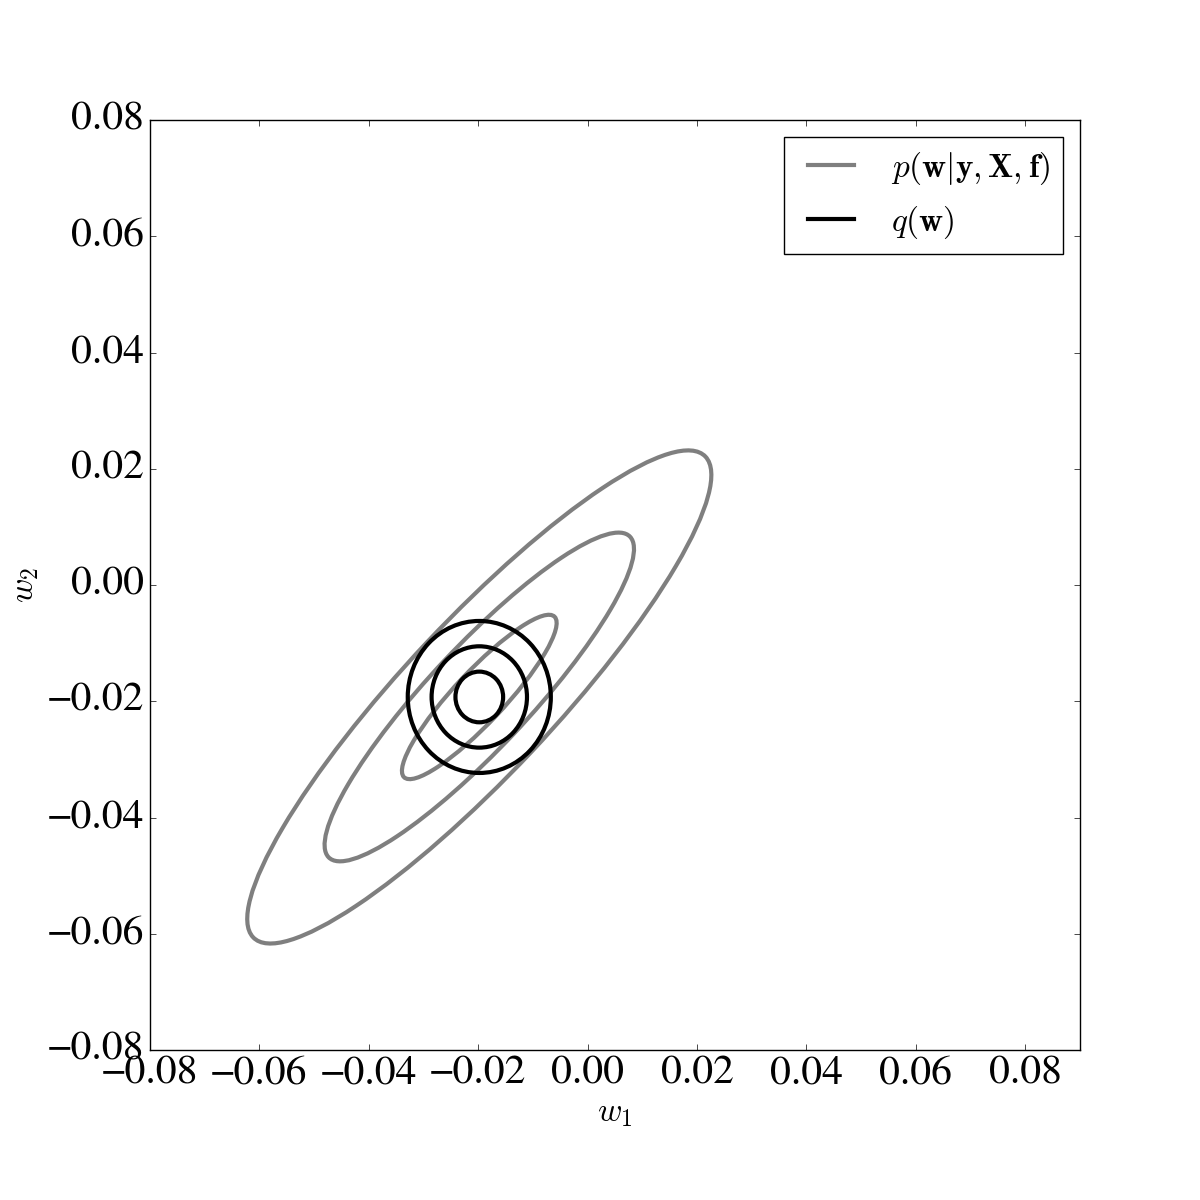
\includegraphics[width=\linewidth]{./plots/mf.pdf}

\endminipage\hfill
\minipage{0.32\textwidth}
\caption*{\textit{б}}
 
  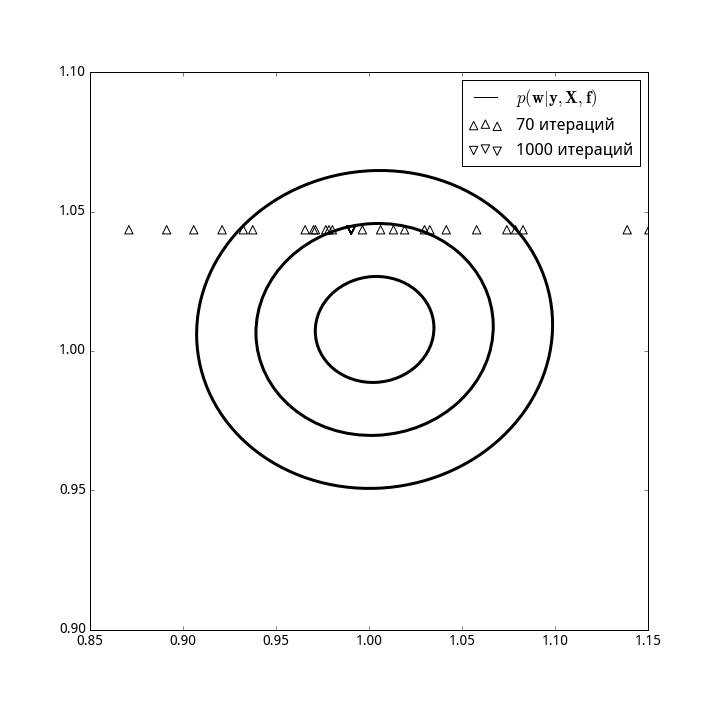
\includegraphics[width=\linewidth]{./plots/sgd.pdf}
 \endminipage\hfill
\minipage{0.32\textwidth}%
 \caption*{\textit{в}}

  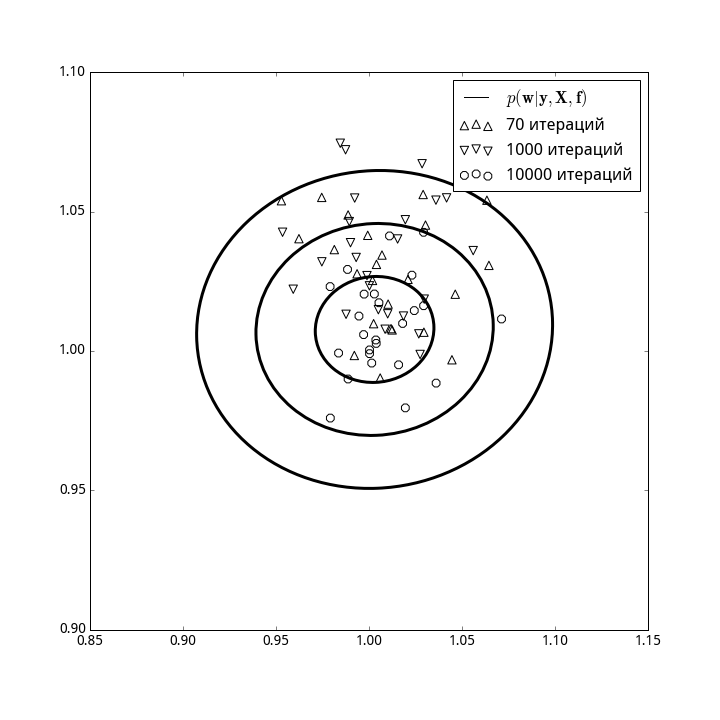
\includegraphics[width=\linewidth]{./plots/lang.pdf}
\endminipage\hfill
  \caption{}
\label{fig:var}
\end{figure}

\begin{figure}[tbh!]


\minipage{0.32\textwidth}
\caption*{\textit{а}}
\includegraphics[width=1.0\textwidth]{./plots/boston/rmse_data2.pdf}
\endminipage\hfill
\minipage{0.32\textwidth}
\caption*{\textit{б}}
\includegraphics[width=1.0\textwidth]{./plots/protein/rmse_data2.pdf}

\endminipage\hfill
\minipage{0.32\textwidth}%
\caption*{\textit{в}}
\includegraphics[width=1.0\textwidth]{./plots/msd/rmse_data2.pdf}

\endminipage
\caption{}
\label{fig:noise_in_data}
\end{figure}

\newpage
%Подрисуночные подписи к ст. Бахтеева, Стрижова. 
Рис. 1. Аппроксимация распределения \textit{а}) нормальным распределением, \textit{б}) распределением,
полученным с помощью градиентного спуска, \textit{в}) с использованием стохастической динамики Ланжевена.
\\~\\
Рис. 2. Возмущение выборки для однослойных нейросетей: \textit{а}) Boston Housing, \textit{б}) Protein, \textit{в}) MSD.

\end{document}
